\chapter{Epidemiological Modelling}

In order to study the behaviour and characteristics of disease spread and
eradication, compartmental epidemiological models have been developed. They
seek to simplify the dynamics of a disease down to a mathematically
representable form. Inference on these models allow for an understanding of how
the modelled disease spreads, and allows an assessment of how effective
differing disease interventions (such as treatments or vaccinations) may be
without the need for large long term trials. Models can also simulate various
scenarios such as increases or decreases in viral transmission.

Simple compartmental disease models assume individuals can be only be in one of
a finite number of states (which are called compartments). These compartments
usually correspond to a state of disease. Some simple common compartments
include: \begin{itemize}
    \item $S$ - Susceptable: at risk of contracting the disease
    \item $E$ - Exposed: contracted the disease but not yet transmitting it
    \item $I$ - Infectious (also called Infected): at risk of transmitting the
          disease
    \item $R$ - Recovered: neither at risk of contracting or transmitting the
          disease.
\end{itemize}

\begin{figure}[htbp]
    \centering
    \begin{subfigure}[b]{0.18\textwidth}
        \begin{tikzpicture}[thick]
            \node[draw, minimum size=0.8cm] (S) {$S$};
            \node[draw, right=of S, minimum size=0.8cm] (I) {$I$};
            \draw[->] (S) edge[in = 160, out = 20] node
            [midway, label=above:{$\lambda_t$}] (lambda) {} (I);
            \draw[->] (I) edge[in = 340, out = 200] node
            [midway, label=below:{$\gamma$}] (gamma) {} (S);
            \draw[->, dashed, ruby] (I) edge[in = 45, out = 90] (lambda);
            % \draw (current bounding box.south east) rectangle
            % (current bounding box.north west);
        \end{tikzpicture}
        \caption{$SIS$ model}\label{fig:SIS_model}
    \end{subfigure}%
    \hfill%
    \begin{subfigure}[b]{0.18\textwidth}
        \begin{tikzpicture}[thick]
            \node[draw, minimum size=0.8cm] (S) {$S$};
            \node[draw, right=of S, minimum size=0.8cm] (I) {$I$};
            \draw[->] (S) edge node [midway, label=above:{$\lambda_t$}]
            (lambda) {} (I);
            \draw[->, dashed, ruby] (I) edge[in = 270, out = 225] (lambda);
            \node[above=of S] (mu) {};
            \node[below=of S] (S_nu) {};
            \node[below=of I] (I_nu) {};
            \draw[->] (mu) edge node [midway, label=left:{$\mu$}] () {} (S);
            \draw[->] (S) edge node [midway, label=left:{$\nu$}] () {} (S_nu);
            \draw[->] (I) edge node [midway, label=left:{$\nu + \gamma$}] () {}
            (I_nu);
            % \draw (current bounding box.south east) rectangle
            % (current bounding box.north west);
        \end{tikzpicture}
        \caption{$SI$ with demography model}\label{fig:SI_demog_model}
    \end{subfigure}%
    \hfill%
    \begin{subfigure}[b]{0.45\textwidth}
        \begin{tikzpicture}[thick]
            \node[draw, minimum size=0.8cm] (S) {$S$};
            \node[draw, minimum size=0.8cm, right=of S] (E) {$E$};
            \node[draw, minimum size=0.8cm, right=of E] (I) {$I$};
            \node[draw, minimum size=0.8cm, right=of I] (R) {$R$};
            \draw[->] (S) edge node [midway, label=above:{$\lambda_t$}]
            (lambda) {} (E);
            \draw[->] (E) edge node [midway, label=above:{$\sigma$}]
            (sigma) {} (I);
            \draw[->] (I) edge node [midway, label=above:{$\gamma$}]
            (r) {} (R);
            \draw[->, dashed, ruby] (I) edge[in = 270, out = 270] (lambda);
            % \draw (current bounding box.south east) rectangle
            % (current bounding box.north west);
        \end{tikzpicture}
        \caption{$SEIR$ model}\label{fig:SEIR_model}
    \end{subfigure}%
    \caption{
        Some simple model schematics, with varying numbers of compartments: $S$
        (susceptable), $E$ (exposed), $I$ (infectious) and $R$ (recovered). The
        force of infection $\lambda_t$ is usually a function of $I_t$, depicted
        by the dashed red lines. $\mu$ and $\nu$ are natural birth and death
        rates respectively. $\gamma$ is the rate of progression out of the
        infectious state. In each of these models the physical interpretation
        differs slightly. In the $SIS$ and $SEIR$ models, it is the rate at
        which individuals move from infectious to susceptable again or into
        lifelong immunity, whereas in the $SI$ with demography model, it can be
        interpreted as the increase to the rate of death attributable to
        disease induced mortality. $\sigma$ is the rate of progression from a
        state of latent infection to becoming infectious.
    }\label{fig:simple_models}
\end{figure}

The number of people in each compartment at time $t$ is a (possibly
non-deterministic) function of time $t,$ which we indicate as a subscript $t$
(eg.\ $S_t$ is the number of susceptibles at time $t$). Models are routinely
described by the compartments they contain. For example, an $SIS$ model, is a
model with the susceptable and infectious compartments. Recovering from the
infection leaves you susceptible to reinfection (for example most sexually
transmitted diseases \parencite[56]{keeling_modeling_2008}), and is graphically
depicted in Figure \ref{fig:SIS_model}.

Furthermore we can also include demography into a compartmental model. Diseases
that infect the individual until the time of death such as bovine spongiform
encephalopathy (BSE commonly known as mad cow disease) may be modelled using an
$SI$ model with demography (birth and death rates), as depicted in Figure
\ref{fig:SI_demog_model} \parencite{hagenaars_epidemiological_2006}.

Childhood diseases such as varicella (chickenpox) which give lifetime immunity
after infection can be modelled using an $SEIR$ model (see Figure
\ref{fig:SEIR_model}), particularly when modelling a local outbreak setting
(for example \cite{zha_research_2020} used the $SEIR$ model to model a school
outbreak of varicella). Not including demograpy is usually appropriate when
disease induced mortality is low.

The number (and names) of compartments can be extended and configured as
needed, and compartments could be added for vaccinated individuals, quarantined
individuals and so on. By convention $N_t$ (often simply $N$ in models with a
closed population) is the total number of individuals in the model, the sum of
all compartments.

\section{Deterministic ODE models}

Diseases are often simulated as deterministic ordinary differential equations.
For the examples below we assume that the force of infection $\lambda_t$ is
proportional to the number of people in $I$, such that
$\lambda_t := \beta \frac{I_t}{N_t}.$ $\beta$ can be interpreted as the average
number of people that an individual interacts with per day in a way such that
disease would be spread in that interaction per unit of time $t$. This is
sometimes called the effective contact rate. Therefore since $\frac{I_t}{N_t}$
is the probability that a randomly selected individual is infectious,
$\beta \frac{I_t}{N_t}$ can be interpreted as the average number of people that
a person interacts with each day who are infectious in a way that they would
pass on the infection. In different diseases $\beta$ varies dramatically, as
some diseases need prolonged exposure or sexual contact to transmit, whereas
some are very highly transmittable, and so will have very low $\beta.$
Implicitly there is also a (sometimes poor) assumption of complete uniformly
random mixing of people. Note that for this thesis we assume that $\beta$ is
frequency dependent (people interact with the same number of people regardless
of population size) as opposed to density dependent (people interact with a
number of people proportional to population size, in which case
$\lambda := \beta I_t.$).

The $SIS$ model depicted in Figure \ref{fig:SIS_model}, the ordinary different
equations (ODEs) governing the model could be \begin{align}
    \frac{\diff S_t}{\diff t} = & \, -\lambda S_t + \gamma I_t = -\beta \frac{I_t}{N}S_t + \gamma I\label{eq:SIS_1} \\
    \frac{\diff I_t}{\diff t} = & \, \lambda S_t - \gamma I_t = \beta \frac{I_t}{N}S_t - \gamma I\label{eq:SIS_2}.
\end{align}

With a stated assumption that population size is closed, equation \ref{eq:SIS_1} fully describes the model.

The system of ODEs that describe the $SI$ with demography model is \begin{align}
    \frac{\diff S_t}{\diff t} = & \, \mu N_t - \lambda_t S_t - \nu I_t = \mu N_t -\beta \frac{I_t}{N_t}S_t - \nu I \label{eq:SI_1}   \\
    \frac{\diff I_t}{\diff t} = & \, \lambda_t S_t - (\gamma + \nu)I_t = \beta \frac{I_t}{N_t}S_t - (\gamma + \nu) I\label{eq:SI_2}.
\end{align} Here is it important to note that $N_t$ is not necessarily constant.

Finally, the system of ODEs that describe the $SEIR$ model is \begin{align}
    \frac{\diff S_t}{\diff t} = & \, - \lambda_t S_t - \nu I                   & = -\beta \frac{I_t}{N}S_t + \gamma I_t \label{eq:SEIR_1} \\
    \frac{\diff E_t}{\diff t} = & \, \lambda_t S_t - \omega E_t                & = \beta \frac{I_t}{N}S_t - \omega I_t \label{eq:SEIR_2}  \\
    \frac{\diff I_t}{\diff t} = & \, \omega E_t - \gamma I_t \label{eq:SEIR_3}                                                            \\
    \frac{\diff R_t}{\diff t} = & \, \gamma I_t \label{eq:SEIR_4}
\end{align}

\begin{figure}[htbp]
    \centering
    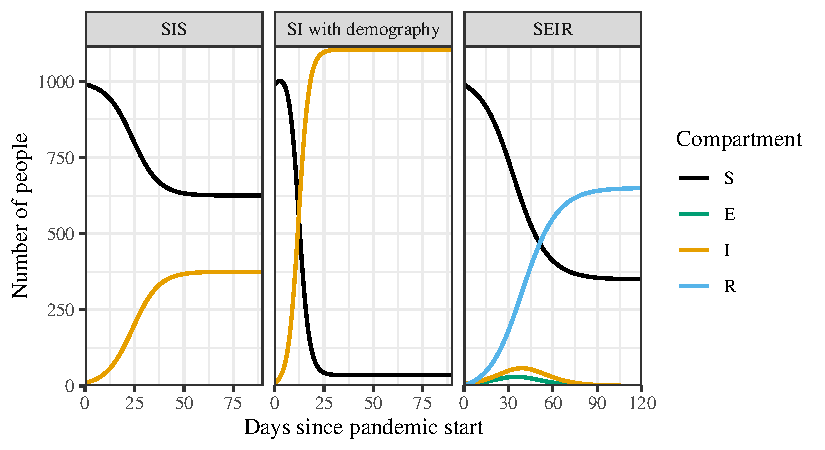
\includegraphics{ODE_plots.pdf}
    \caption{
        Solutions to the ordinary differential equations describing the models 
        depicted in Figure \ref{fig:simple_models}. The initial infectious 
        population was $I_0 = 10,$ with $S_0 = 990.$ In the $SEIR$ model, 
        $E_0 = R_0 = 0.$ For all models $\beta = 0.4.$ For the $SIS$ and $SI$
         model with demography $\gamma = 1/4.$ For the $SI$ model with 
         demography $\mu = 0.012,$ and $\nu = 0.0012.$ For the $SEIR$ model, 
         $\gamma = 1/90,$ and $\sigma = 1/2.$
    }
         \label{fig:ODE_outputs}
\end{figure}

After specifying the initial for each compartment the ordinary differential equations have a deterministic output, such as in \ref{fig:ODE_outputs}.

\section{Stochastic models}

\subsection*{Motivating the form of the stochastic model}

To establish a relationship between the deterministic and stochastic disease models, we first need to establish Poisson point processes and their properties.

\begin{definition}[Poisson Point Process]\label{def:ppp}
    $\{\N(t)\}_{t\geq0}$ is a \emph{(stationary) Poisson point process} with intensity $\lambda$ if \begin{enumerate}
        \item $\N(0) = 0$
        \item $\N(t_1) - \N(t_0), \N(t_2) - \N(t_1), \dots, \N(t_n) - \N(t_{n-1})$ are independent for $0 \leq t_0 < t_1 < \dots < t_{n-1} < t_n $
        \item $\N(t_2) - \N(t_1) \sim \Pois(\lambda(t_2 - t_1)), 0 \leq t_1 < t_2.$
    \end{enumerate}
\end{definition}

Deterministic ODE models are appropriate to study a kind of aggregate disease spread behaviour, and well approximate real world behaviour when the numbers in each compartment are large, however at the start of an epidemic, when the number of infected individuals is small the behaviour of the epidemic may vary significantly. It is possible that if the average number of people that an infectious individual infects near the beginning of the epidemic (formally referred to as $R_0$) is close to 1, then the disease may die out or become stable. Under the deterministic $SIS$ model described by equations \ref{eq:SIS_1} and \ref{eq:SIS_2}, consider the model at time $t^*$ the instantaneous rate at which $S$ is decreasing is $\beta \frac{I_{t^*}}{N} S_{t^*}.$ In other words, one individual leaves the $S$ compartment every $\beta \frac{I_{t^*}}{N} S_{t^*}$ units of time. We can consider a Poisson point process $\{\N_1(t - t^*)\}_{t\geq t^*}$ with intensity $\beta \frac{I_{t^*}}{N} S_{t^*}$ corresponding to the count of the number of individuals who have left $S$ and entered $I$ $t$ units of time since $t^*.$ $$\frac{\diff \E(\N_1(t^*))}{\diff t^*} = \lim_{\delta \to 0}\frac{\E{(\N(t^* + \delta) - \N(t^*))}}{\delta} = \frac{\beta \frac{I_{t^*}}{N} S_{t^*}(t^* + \delta - t^*)\beta \frac{I_{t^*}}{N} S_{t^*}}{\delta} = \beta \frac{I_{t^*}}{N} S_{t^*}.$$

Under the same deterministic formulation of the model, the instantaneous rate into $S$ at $t^*$ is $\gamma I_{t^*}.$ Therefore as above we can construct a Poisson point process $\{\N_2(t - t^*)\}_{t\geq t^*}$ with rate $\gamma I_{t^*}$ describing the number of recoveries from $I$ to $S,$ with $\frac{\diff \E(\N_2(t^*))}{\diff t^*} = \gamma I_{t^*}.$ Combining the two processes, we can see that the rate of change in the average number of people in $S$ is $$\frac{\diff \E(\N_2(t^*) - \N_1(t^*))}{\diff t^*} = \frac{\diff \E(\N_2(t^*)) - \diff \E(\N_1(t^*))}{\diff t^*} = -\beta \frac{I_t}{N}S_t + \gamma I = \frac{\diff S_t}{\diff t}.$$

% \begin{definition}[Markov Chain]
%     A set of random variables $\{X_i\}_{i\in\mathcal{I}}$ is Markov if $\Pr(X_{i})$
% \end{definition}

Therefore we can create a stochastic model where the local average in each compartment matches the behaviour of the ODE model at the same state. We do this first by formulating the model as a random vector $\{\mathbf{C}_t\}_{t\geq 0} = \{C_1(t), C_2(t), \dots, C_n(t)\}_{t\geq 0}$ where $C_i:\mathbb{R} \to \mathbb{N}\cup\{0\},$ is the number of people in compartment $C_i,$ and for any fixed $t$, $\{C_1(t), C_2(t), \dots, C_n(t)\}$ is a random variable describing the state of the model. For example in a model with $S$ and $I$ compartments, $\{\mathbf{C}_t\}_{t\geq 0}:=\{S_t, I_t\}_{t\geq 0}.$ $\{\mathbf{C}_t\}_{t\geq 0}$ is a continuous time Markov chain (see Definition \ref{Markov_chains}) with transition kernel corresponding to the rates of the model. For example, in the $SI$ model with demography in Figure \ref{fig:SI_demog_model} the transition rates are: \begin{itemize}
    \item $\{s, i\}$ to $\{s + 1, i\}$ has rate $\mu (s + i)$
    \item $\{s, i\}$ to $\{s - 1, i\}$ has rate $\nu s$
    \item $\{s, i\}$ to $\{s - 1, i + 1\}$ has rate $\beta \frac{i}{i+s}s$
    \item $\{s, i\}$ to $\{s, i - 1\}$ has rate $(\nu + \gamma) i.$
\end{itemize}

We can interpret each transition as a seperate events, each behaving as independent Poisson point processes until the time of the first transition. Therefore at time $t^*$ we have the Poisson point processes: \begin{itemize}
    \item $\{\mathcal{E}_1(t)\}_{t\geq 0}:$ the number of births into $S$ after time $t^*$ with intensity $\mu N_{t^*}$
    \item $\{\mathcal{E}_2(t)\}_{t\geq 0}:$ the number of deaths in $S$ after time $t^*$ with intensity $\nu S_{t^*}$
    \item $\{\mathcal{E}_3(t)\}_{t\geq 0}:$ the number of infections after time $t^*$ with intensity $\beta \frac{I_{t^*}}{N_{t^*}} S_{t^*}$
    \item $\{\mathcal{E}_4(t)\}_{t\geq 0}:$ the number of deaths from $I$ after time $t^*$ with intensity $(\nu + \gamma) I_{t^*}.$
\end{itemize}

\begin{theorem}[Sums of Independent Poisson Point Processes]\label{thm:sum_ppp}
    Given independent Poisson point processes $\{\N_1(t)\}_{t\geq0},
        \{\N_2(t)\}_{t\geq0}, \dots,  \{\N_n(t)\}_{t\geq0},$ with intensities
    $\lambda_1, \lambda_2, \dots, \lambda_n,$
    $$\{\N(t)\}_{t\geq0} := \{\N_1(t) + \N_2(t) + \dots + \N_n(t)\}_{t\geq0}$$ is a Poisson point process with intensity $\lambda_1 + \lambda_2 + \dots +
        \lambda_n.$
\end{theorem}

\begin{proof}
    We show that
    $\{\N(t) := \{\N_1(t) + \N_2(t) + \dots + \N_n(t)\}_{t\geq0}\}$ meets each
    component of Definition \ref{def:ppp}.
    \begin{enumerate}
        \item $\N(0) := \N_1(0) + \N_2(0) + \dots + \N_n(0) = 0$ since
              $\N_i(0) = 0$ by definition of a Poisson point process.
        \item We show that $\N(t_1) - \N(t_0), \N(t_2) - \N(t_1), \dots,
                  \N(t_n) - \N(t_{n - 1})$
              with $0 \leq t_0 < t_1 < \dots < t_n$ are independent.
              $$\N(t_i) - \N(t_{i - 1})
                  = \underset{X_{i1}}
                  {\underbrace{[\N_1(t_i) - \N_1(t_{i - 1})]}}
                  + \underset{X_{i2}}
                  {\underbrace{[\N_2(t_i) - \N_2(t_{i - 1})]}} + \dots
                  + \underset{X_{in}}
                  {\underbrace{[\N_n(t_i) - \N_n(t_{i - 1})]}}$$
              $X_{ik}$ is independent of $X_{j\ell}$ for $k \neq \ell$ since
              $\N_k$ and $\N_\ell$ are independent processes. $X_{ik}$ is
              independent of $X_{jk}$ for $i\neq j$ by the second property
              of Definition \ref{def:ppp}. Therefore all $X_{ik}$ are
              independent of $X_{j\ell}$ for $i\neq j,$ and all $j, k.$
              Hence
              $\N(t_1) - \N(t_0), \N(t_2) - \N(t_1), \dots,
                  \N(t_n) - \N(t_{n - 1})$
              with $0 \leq t_0 < t_1 < \dots < t_n$ are independent.
        \item For fixed $t_1 < t_2,$ and $i \in \{1, 2, \dots, n\},$
              $$\N_i(t_2) - \N_i(t_1) \sim \Pois((t_2 - t_1)\lambda_i).$$
              Consider the associated moment generating function of
              $\N_i(t_2) - \N_i(t_1),$
              $$M_i(z) := \exp(\lambda_i(t_2 - t_1)(\exp(z) - 1)).$$
              Therefore the moment generating function of
              $$\N(t_2) - \N(t_1) =
                  [\N_1(t_2) - \N_1(t_1)] + [\N_2(t_2) - \N_2(t_1)] + \dots
                  + [\N_n(t_2) - \N_n(t_1)]$$ is
              $$ M(z) := \prod_{i = 1}^n M_i(z) =
                  \exp[
                      (\lambda_1 (t_2 - t_1) + \lambda_2 (t_2 - t_1) + \dots
                      + \lambda_n (t_2 - t_1))
                      (\exp(z) - 1)
                  ].$$
              Therefore
              $\N_1(t) + \N_2(t) + \dots + \N_n(t) \sim
                  \Pois((\lambda_1 + \lambda_2 + \dots + \lambda_n) t)$
              by the uniqueness of the moment generating function.
    \end{enumerate}
\end{proof}

\begin{theorem}[Time to First Event in Poisson Point Process]
    \label{thm:next_pp_event}
    Given a Poisson point process $\{\N(t)\}_{t\geq 0}$ with intensity
    $\lambda,$ let $\tau = \inf\{t | \N(t_0 + t) - \N(t_0) = 1, t > 0\}$.
    $\tau \sim \Exp(\lambda)$ for $t_0 \geq 0$
\end{theorem}

\begin{proof}
    $$\Pr(\tau > x) = \Pr(\N(t_0 + x) - \N(t_0) = 0)
        = \frac{(\lambda x)^0e^{-\lambda x}}{0!} = e^{-\lambda x}$$
\end{proof}

By Theorem \ref{thm:sum_ppp} and Theorem \ref{thm:next_pp_event},
$$\{\mathcal{E}(t)\}_{t\geq 0}:=\{\mathcal{E}_1(t) + \mathcal{E}_2(t)
    + \mathcal{E}_3(t) + \mathcal{E}_4(t)\}_{t\geq 0}$$
is a Poisson point process with intensity
$$\mu N_{t^*} + \nu S_{t^*} + \beta \frac{I_{t^*}}{N_{t^*}} S_{t^*}
    + (\nu + \gamma) I_{t^*},$$
and the time to the next event is random variable distributed
$$\Exp(\mu N_{t^*} + \nu S_{t^*}
    + \beta \frac{I_{t^*}}{N_{t^*}} S_{t^*} + (\nu + \gamma) I_{t^*}).$$

\begin{theorem}[Probability of $i$th Poisson Process Generating the Next Event]\label{thm:which_ppp}
    Consider independent Poisson point processes
    $$\{\N_1(t)\}_{t\geq0},\, \{\N_2(t)\}_{t\geq0},\, \dots,\,
        \{\N_n(t)\}_{t\geq0}$$
    having intensities $\lambda_1, \lambda_2, \dots, \lambda_n.$ For fixed
    $t_0,$ let $\tau_i:=\inf\{t | \N(t_0 + t) - \N(t_0) = 1\}.$
    Then
    $$\Pr(\min_i{\tau_i} = \tau_j)
        = \frac{\lambda_j}{\sum_{i = 1}^n \lambda_i}.$$
\end{theorem}
\begin{proof}
    By Theorem \ref{thm:next_pp_event}, $\tau_i \sim \Exp(\lambda_i).$
    Therefore \begin{align*}
        \Pr(\min_i{\tau_i} = \tau_j) = & \int_0^\infty \Pr(\{\tau_i = x\} \cup \bigcup_{j\neq i}\{\tau_j > x\}) \diff x                    \\
        =                              & \int_0^\infty \Pr(\{\tau_i = x\} \cup \bigcup_{j\neq i}\{\tau_j > x\}) \diff x                    \\
        =                              & \int_0^\infty \Pr(\tau_i = x)\times \prod_{j\neq i}\Pr(\tau_j > x) \diff x\tag{by independence}   \\
        =                              & \int_0^\infty \lambda_i\exp(-\lambda_i x) \times \prod_{j\neq i}\exp(-\lambda_j x) \diff x        \\
        =                              & \lambda_i\int_0^\infty \exp(-(\sum_{i = 1}^n\lambda_j) x) \diff x                                 \\
        =                              & \lambda_i\left[\frac{\exp(-(\sum_{i = 1}^n\lambda_j) x)}{\sum_{i = 1}^n\lambda_j}\right]_0^\infty \\
        =                              & \frac{\lambda_i}{\sum_{i = 1}^n\lambda_j}
    \end{align*}
\end{proof}

\section{Doob-Gillespie Algorithm}

All of this leads naturally to a common method of simulating the stochastic model. The Doob-Gillespie algorithm (often just called the Gillespie algorithm) is an algorithm that simulates a stochastic realisation of a model given a set of starting conditions.

\begin{algorithm}
    \caption{The Doob-Gillespie Algorithm}\label{alg:doob}
    \begin{algorithmic}[1]
        \State Initialise time $t \gets 0$ and initial state of the model $\mathbf{C}(0) := \{C_1(0), C_2(0), \dots, C_n(0)\}$
        \While{termination condition not met}
        \State Calculate intensities $\lambda_i$ for all possible events $\mathcal{E}_i$
        \State Calculate total intensity $\lambda = \sum_i \lambda_i$
        \State Generate $\Delta t \sim \Exp(\lambda)$
        \State Choose event $\mathrm{E}_i$ with probability $\frac{\lambda_i}{\lambda}$
        \State Update time $t \gets t + \Delta t$
        \State Update state of $\mathbf{C}(t + \delta t) \gets \mathbf{C}(t) + \text{ change in state due to event } \mathcal{E}_i$
        \EndWhile
    \end{algorithmic}
\end{algorithm}

\begin{figure}[htbp]
    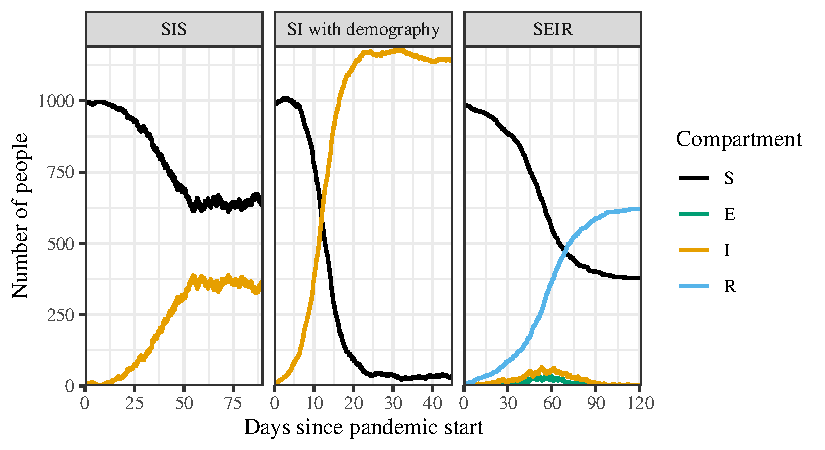
\includegraphics{doob_plots.pdf}
    \caption{Exact stochastic simulations of the 3 different models using Algorithm \ref{alg:doob}. The parameters used were identical to those in Figure \ref{fig:ODE_outputs}}\label{fig:doob_outputs}
\end{figure}

\section{\texorpdfstring{$\tau$}{Lg}-leaping}

$\tau$-leaping exploits the local Poisson point process like behaviour of epidemiological models. Consider the SIS model, when $S_t = I_t = 10000.$ Events happen at a very high rate, meaning the $\Delta t$ found in each step of the Doob-Gillespie algorithm will be very small, but the rates also change a negligible amount after each event (compare $\gamma\times 10000$ to $\gamma\times 10001$ or $\gamma\times 9999$). Therefore we can approximate the number of events in a short time period $\tau$ as a Poisson point process with the total intensity $\lambda = \sum_i \lambda_i$ at time $t,$ with the probability of any one event having the same probability as above of $\frac{\lambda_i}{\lambda}.$ Therefore we have the following algorithm.

\begin{algorithm}
    \caption{$\tau$-Leaping Algorithm}
    \label{alg:tau_leaping}
    \begin{algorithmic}[1]
        \State Initialise time $t \gets 0$ and initial state of the model $\mathbf{C}(0) := \{C_1(0), C_2(0), \dots, C_n(0)\}$
        \While{termination condition not met}
        \State Calculate intensities $\lambda_i$ for all possible events $\mathcal{E}_i$
        \State Calculate total intensity $\lambda = \sum_i \lambda_i$
        \State Choose a suitable time step $\tau$ (this can be deterministic or adaptive)
        \State Calculate Poisson random variable $X \sim \text{Poisson}(\lambda)$
        \For{$i$ in 1 to $X$}
        \State Choose event $\mathrm{E}_i$ with probability $\frac{\lambda_i}{\lambda}$
        \State Update state of $\mathbf{C}(t + \tau) \gets \mathbf{C}(t) + \text{ change in state due to event } \mathcal{E}_i$
        \EndFor
        \State Update time $t \gets t + \tau$
        \EndWhile
    \end{algorithmic}
\end{algorithm}

% \section{Individual based models}